
We evaluate the performance of \seidr{} from several angles.
On classification, we are interested in the accuracy of CCA detection using IAT histograms, the time taken to train a model, and the required time to classify a flow.
In the \emph{2-class} problem, we investigate whether it is possible to separate TCP \emph{BBR} from \emph{Cubic} using IAT histograms as the input data, while in the \emph{4-class} problem we extend this to include \emph{Reno} and \emph{Vegas}.
We compare our work against \textcite{DBLP:conf/icccn/HagosEYK18} in this regard.
On deployment, we investigate the bandwidth and memory requirements imposed by \seidr{}.

% Evaluation ideas for the system:
% \begin{enumerate}
%     \item Dataplane calculation: how many histograms can we do reasonable, how much memory space it needs
%     \item Show data reduction rates with dataplane aggregation - this depends on windowing as well - 1 ms, 100 ms - just back of the envelope calculation with some visualization. Assuume: per-flow histograms, packet size of 1500B, 100Gbit/s worth of traffic. 
% \end{enumerate}{}


% Evaluation ideas for the classification use-case:
% \begin{enumerate}
%     \item CNN classifier accuracy
%     \item CNN vs KNN vs LSTM vs K-means [traning time vs performance scatterplot]
%     \item Timestamp accuracy - importance of nanosecond timing from the dataplane
% \end{enumerate}

\subsection{Datasets}\label{sec:seidr-datasets}
We examine synthetic flows modelling bulk data transfer at various speeds, generated using iPerf3\footnote{\url{https://iperf.fr/}}, and processed using custom P4 firmware.
% Inter-arrival time streams are extracted using custom P4 firmware installed on Netronome Agilio CX 2x40GbE SmartNICs.
% Histograms are generated at classification time from these streams to ensure consistent input data and results between classification techniques and individual trials.
For every pairwise interaction between TCP \emph{BBR}, \emph{Cubic}, \emph{Reno}, and \emph{Vegas}, we capture solo and multiplexed dynamics by running each flow for \SI{3}{\second}, with \SI{2}{\second} of overlap (\ie, the second flow begins at $t=\SI{1}{\second}$).
We observe that the first flow always completes slow-start before multiplexing begins, and by construction we have several unimpeded captures for every flavour.
We do not expect the number/volume of multiplexed flows to substantially alter captured dynamics (\ie, 3 flows at \SI{300}{\mega\bit\per\second} and 2 flows at \SI{200}{\mega\bit\per\second} should both have flows fall to \SI{100}{\mega\bit\per\second}).
Flows in one capture are generated using the same target rate in $\left\{\num{100},\num{200},\dots,\num{1000}\right\}$\si{\mega\bit\per\second}, each perturbed randomly within $\pm\SI{10}{\percent}$ uniformly.
We also control how this rate limit is applied: \emph{wire-limited} traffic uses \texttt{tc} in the Linux kernel to apply rate-limiting, while \emph{application-limited} traffic uses iPerf's builtin mechanisms to control send rate.
Application-limited traffic leads to specific behaviour in \emph{BBR} and some other flavours, while wire-limited traffic creates loss events as the rate grows too high.
\num{10} such captures are recorded for each $(\mathit{CCA}_1,\mathit{CCA}_2,\mathit{speed},\mathit{limiter})$ tuple, and generated flows are labelled accordingly.

IAT streams are broken down into overlapping sequences of the required length, before being histogrammed as required into \num{100} buckets over \SIrange{0}{1}{\milli\second}.
The use of overlapping sequences extends the training and testing sets significantly, while ensuring that larger sequences don't result in a far smaller training corpus.
Cross-validation occurs on a per-flow basis rather than per-sequence, \ie sequences from the same flow must only appear in \emph{either} the test or training set to preserve stringent data hygiene and prevent adjacent sequences from inducing overfitting.
All classifier evaluation which follows uses 4-fold cross-validation.
The data is comprised of \num{4994} flows (\num{832} in \emph{2-class}), or \numrange{18}{31} million sequences (\numrange{3.2}{5.2} million in \emph{2-class}).

\subsection{Experimental Setup}
All experiments were executed on Ubuntu 18.04.4 LTS (GNU/Linux 4.15.0-96-generic x86\_64), using a 4-core Intel Core i7-6700K (clocked at \SI{4.2}{\giga\hertz}) and \SI{32}{\giga\byte} of RAM.
CNN training was performed using Nvidia RTX 2080Ti cards (\SI{11}{\giga\byte} GDDR6 VRAM).
For the dataplane, we used multiple Netronome Agilio CX 2x40GbE SmartNICs using 40GbE connections between source and destination hosts.
% All code underpinning these findings is available on a public
% repository

% All our experiments are run on ESnet's test setup, using production servers with Intel Xeon Gold 6242 CPUs clocked at \SIrange{2.8}{3.9}{\giga\hertz} (32 cores) and \SI{793}{\giga\byte} of RAM.

\subsection{Classification Performance}
In the \emph{2-class} formulation, we observe from \cref{fig:2c-results} that CNN performance increases slightly with the length of the input sequence for classifying application-limited traffic.
Our CNN-based detection has a peak F1-score of \num{0.965} for application-limited traffic, and \num{0.894} when wire-limited.
This increase does not extend towards full-sequence histograms, which are hampered by having 6 orders of magnitude fewer training samples.
While very effective, $k$-NNs come with significant memory cost.
By design, the entire dataset must be kept in memory: for length \num{500}, this equates to \SI{1.5}{\gibi\byte} of training data.
Naturally, this is undesirable for many network deployments, where easy relocation of inference may be key.

\begin{figure}
    \centering
    \resizebox{0.7\linewidth}{!}{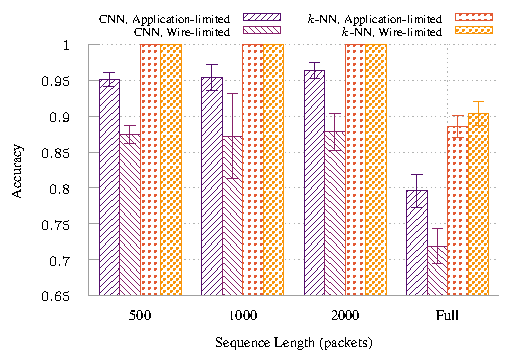
\includegraphics{plots/seidr/2class-results.pdf}}
    \caption{Accuracy of $k$-NN and CNN classifiers when classifying \emph{BBR} and \emph{Cubic} TCP traffic from IAT histograms, trained  over various sequence lengths.}
    \label{fig:2c-results}
\end{figure}

\begin{figure}
    \centering
    \resizebox{0.7\linewidth}{!}{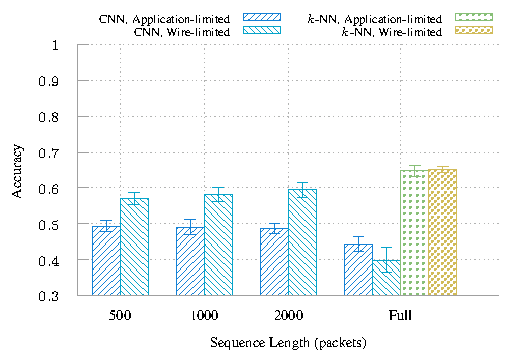
\includegraphics{plots/seidr/4class-results.pdf}}
    \caption{Accuracy of $k$-NN and CNN classifiers when classifying \emph{BBR}, \emph{Cubic}, \emph{Reno}, and \emph{Vegas} TCP traffic from IAT histograms, trained and tested on various sequence lengths.}
    \label{fig:4c-results}
\end{figure}

\Cref{fig:4c-results} shows in the \emph{4-class} case that we observe a sharp loss in classification accuracy, peaking at \SI{59.5 +- 2}{\percent} for CNNs and \SI{64.5 +- 1.6}{\percent} for $k$-NN.
This suggests that IAT histograms don't generalise as an effective feature for other TCP flavours.
Exploratory work with LSTMs on IAT streams confirmed that this persists before aggregation.
Likewise, exclusive pairwise training did not lead to an increase in accuracy.
However, \cref{fig:4c-cnn-conf} shows that timing information remains key in separating BBR from its predecessors to a high degree of accuracy, confirming our hypothesis that its \emph{timer}-based (rather than \emph{cwnd}-based) design allows for this detection.
If this marker were present between \emph{loss}- and \emph{delay}-based variants, then we'd also see high predictive power over \emph{Vegas} traffic.
Breaking down these confusion matrices by rate limit type sheds still more light.
In \cref{fig:4c-cnn-conf-app}, application-limited data transfers are almost indistinguishable using these metrics (aside from \emph{Vegas}), while \cref{fig:4c-cnn-conf-tc} reveals that IATs hold some discriminative power for wire-limited Cubic traffic.
Note that \emph{4-class} $k$-NN experiments on all but full sequences required excessive memory and classification time, and so are excluded.
While full-sequence $k$-NNs outperform all examined CNNs on this task (respective peak F1-scores \num{0.697} vs.\@ \num{0.486}), we observe that these reduce $\mathit{F1}_\mathit{BBR}$ from \num{0.935} to \num{0.810}.

\begin{figure}
    \centering
    \begin{subfigure}[b]{0.49\linewidth}
    \centering
    \resizebox{1.0\linewidth}{!}{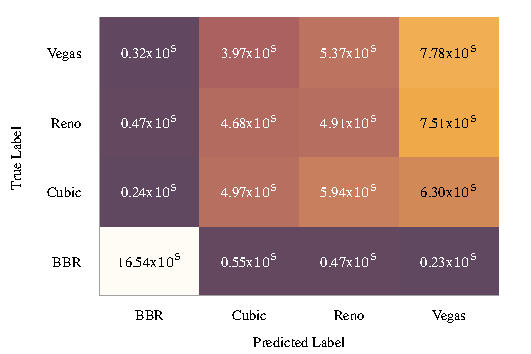
\includegraphics{plots/seidr/cnn-histo-app-confusion-2000.pdf}}
    \subcaption{\emph{Application-limited}.\newline ${\mathit{F1}_\mathit{BBR}=0.935}$, ${\mathit{F1}=0.486}$.}
    \label{fig:4c-cnn-conf-app}
    \end{subfigure}%
    \begin{subfigure}[b]{0.49\linewidth}
    \centering
    \hspace{-1.5em}
    \resizebox{1.0\linewidth}{!}{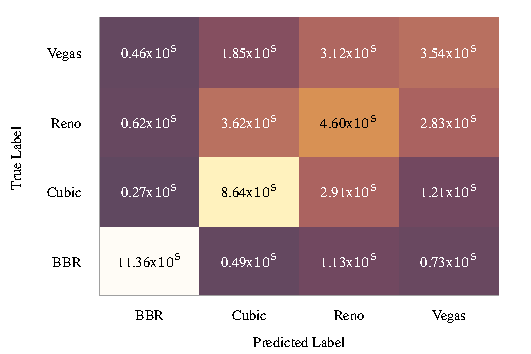
\includegraphics{plots/seidr/cnn-histo-tc-confusion-2000.pdf}}
    \caption{\emph{Wire-limited}.\newline ${\mathit{F1}_\mathit{BBR}=\num{0.893}}$, ${\mathit{F1}=\num{0.573}}$. 
    % Notably, ${\mathit{F1}_\mathit{Cubic}=\num{0.625}}$.
    }
    \label{fig:4c-cnn-conf-tc}
    \end{subfigure}
    
    \caption{Confusion matrices for a CNN on the \emph{4-class} problem, \num{2000}-packet length sequences. Brighter entries along the diagonal indicate correct classifications. BBR remains easy to distinguish regardless of the rate limit mechanism, while Cubic is slightly more distinct for wire-limited traffic.}
    \label{fig:4c-cnn-conf}
\end{figure}

We contrast our work with that of \textcite{DBLP:conf/icccn/HagosEYK18}, who employ CNNs to predict \emph{cwnd} size for any flow from its stream of bytes-in-flight measurements.
On detection of a loss event the \emph{multiplicative decrease} $\beta$ is measured from estimated \emph{cwnd}s, from which the CCA may be classified.
In identifying TCP \emph{BIC}, \emph{Cubic}, and \emph{Reno}, they achieve \SI{95}{\percent} accuracy, which outperforms \seidr{} on \emph{cwnd}-based CCAs.
% ??Their work aims to capture the dynamics of loss-based CCAs, but we claim that the shared factor is in fact the reliance upon a sliding congestion window.
Yet their approach cannot work for detecting \emph{BBR}. 
\emph{BBR} is not based upon the notion of a sliding congestion window, so there is no parameter $\beta$ to infer.
Although IAT histograms are suitable for \emph{BBR} detection due to the intrinsic properties of its algorithm, we envision that our approach could be augmented by using a negative \emph{BBR} classification to trigger \emph{cwnd} estimation.
Having seen that some predictive power is preserved for \emph{cwnd}-based CCAs, we expect that this will increase the accuracy of a universal classifier.
It is important, however, that this step be taken adaptively; this incurs higher resource requirements for bytes-in-flight tracking and for efficient handling of potential return-path asymmetry.
\seidr{} on its own does not add such overheads or operational complexity, and does not require sight/detection of \emph{cwnd} adjustments.

\subsection{Training and Inference Costs}
\begin{table}[]
    \centering
    \caption{Training and inference costs on our test server.}
    \resizebox{0.8\linewidth}{!}{\begin{tabular}{@{}cccccc@{}}\toprule
         Family & Online/Subsequence & $n_\mathit{classes}$ & Train & Test & Memory \\ \midrule
        CNN & \checkmark & 2 & \SI{43 +- 2}{\minute} & \SI{49.1 +- 9.2}{\micro\second} & \SI{409.76}{\kibi\byte} \\
          & \checkmark & 4 & \SI{243 +- 2}{\minute} & \SI{50.5 +- 1.7}{\micro\second} & \SI{410.27}{\kibi\byte} \\
          & \xmark & 2 & \SI{1.82 +- 0.47}{\second} & \SI{161.3 +- 3.9}{\micro\second} & \SI{409.76}{\kibi\byte} \\
          & \xmark & 4 & \SI{7.94 +- 0.5}{\second} & \SI{137.7 +- 1.2}{\micro\second} & \SI{410.27}{\kibi\byte} \\

        $k$-NN & \checkmark & 2 & \SI{21.4 +- 1.2}{\minute} & \SI{323 +- 69}{\micro\second} & \SI{2.1}{\gibi\byte} \\
          & \checkmark & 4 & --- & --- & \SI{12.58}{\gibi\byte} \\
          & \xmark & 2 & \SI{0.2 +- 0.006}{\second} & \SI{54.0 +- 0.3}{\micro\second} & \SI{332.8}{\kibi\byte} \\
          & \xmark & 4 & \SI{2.2 +- 0.04}{\second} & \SI{517.0 +- 5.0}{\micro\second} & \SI{2.0}{\mebi\byte} \\
         \bottomrule
    \end{tabular}}
    \label{tab:train-test-times}
\end{table}

We list typical test and training times for our problem formulations in \cref{tab:train-test-times}.
Training times for $k$-NN include the time taken to load and process the entire training set, and are incurred \emph{every time} the model is started on a new host.
CNNs trained for online analysis (flow subsequences) achieve the lowest per-flow inference times, and are increased during offline analysis due to worse batching and cache behaviour on the smaller data set.
While $k$-NN is effective in many cases, we found it to only be computationally viable when offline (\ie, full-flow histograms), as the entire test data corpus must remain in memory.
A single \emph{4-class} cross-validation fold (\num{2000} packets) required 3 days to train and test over the entire dataset, which we deemed infeasible.
In contrast, while online CNNs take longer to train, they have a considerably lower memory footprint, the training cost is paid only once, and flows may be classified in real-time with milliseconds of observations.

\subsection{Switch Resource Usage}
The implementation of \seidr{} requires an additional table in the ingress pipeline to update buckets, update configuration, and rewrite packets.
Further code space is required to include a configuration packet parser.
Shared configuration data (registers \numrange{1}{5}) requires \SI{42}{\byte} per switch, while each flow requires \SIlist{224;248}{\byte} to store buckets, counters, previous timestamps, and active 5-tuples on IPv4/v6 networks respectively.
On platforms which support hash-table structures, this cost scales linearly with the number of tracked flows.
Otherwise, this requires pre-allocation of an entry for every possible hash value (\eg, \SIrange{14}{15.5}{\mebi\byte} for a \SI{16}{\bit} hash). This small memory requirement fits histogram generation to all devices available today.

\subsection{Quantifying In-Network Data Aggregation}

\begin{figure}
    \centering
    \resizebox{0.95\linewidth}{!}{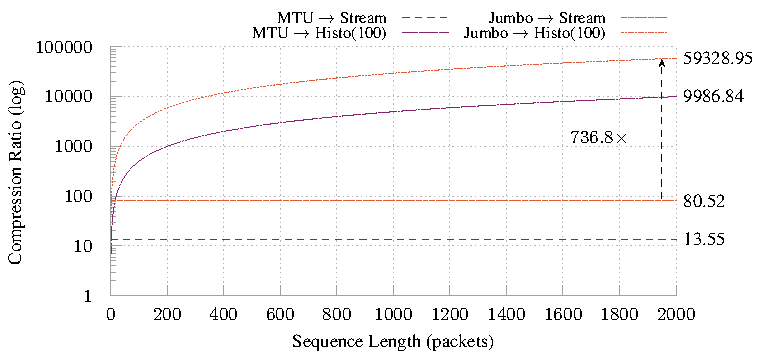
\includegraphics{plots/seidr/compression-v6.pdf}}
    \caption{Compression ratio of \num{100}-bucket histograms and timestamp streams from raw packets on an IPv6 network. As sequence length increases, histograms provide more of an advantage in compression rate, being \SI{736.8}{$\times$} smaller than timestamp streams when analysing \num{2000}-packet sequences.}
    \label{fig:histo-compression}
\end{figure}

% \begin{figure}
%     \centering
%     \resizebox{\linewidth}{!}{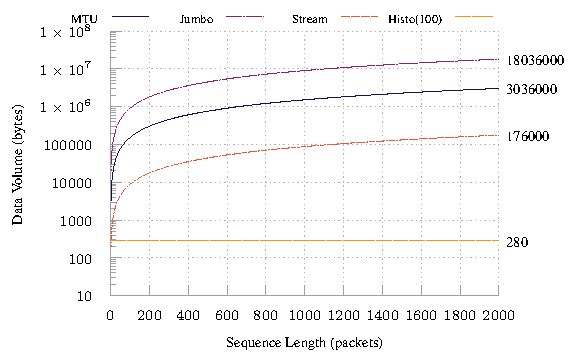
\includegraphics{plots/histo-sz-v6.pdf}}
%     \caption{Data volume of 100-bucket histograms and timestamp streams versus raw packets on an IPv6 network.}
%     \label{fig:histo-sz}
% \end{figure}

\Cref{fig:histo-compression} demonstrates the reduction in data sent from raw mirrored packets, to a stream of measured timestamps/IATs, to \seidr{} histograms on an IPv6 network.
Timing histograms naturally provide a larger data reduction as the amount of measured packets increases, while a per-packet IAT/telemetry stream offers no reduction in packet rate.
Due to this, 100-bucket histograms cause a greater data reduction than per-packet IATs after just 4 packets in a sequence, and consume \SI{736.8}{$\times$} less volume for \num{2000}-packet sequences.

To make this concrete, \SI{100}{\giga\bit\per\second} traffic is reduced to \SI{10.01}{\mega\bit\per\second} additional switch traffic for MTU-size packets, and to \SI{1.69}{\mega\bit\per\second} for jumbo frames.
IAT streams, by comparison, reduce to \SI{7.38}{\giga\bit\per\second} (resp.\ \SI{1.24}{\giga\bit\per\second}).
For a flow at \SI{100}{\mega\bit\per\second}, only \SI{30}{\milli\second} is needed to collect enough packets to make a classification.
Scaling beyond this, packet processing rates are the bottleneck.
As commodity machines and today's stream processors have a reasonable upper bound of $\sim$1M PPS processing capacity~\parencite{DBLP:conf/sigcomm/GuptaHCFRW18}, \seidr{} could scale up to \SI{1}{\tera\bit\per\second} MTU-size packet traffic on one machine, which would correspond to only 333K PPS histogram packets (55.6K PPS if jumbo-size).
Reliably scaling to \SI{10}{\tera\bit\per\second} and beyond requires only that we increase the histogram sequence length to $\ge\num{7000}$ packets.

